%! Author = adrien koumgang tegantchouang
%! Date = 09/07/24

\chapter{Implementation of modular decomposition}\label{ch:implementation-of-modular-decomposition}

Modular decomposition is a powerful technique used to simplify and analyze the structure of graphs by breaking them down into modules.
One of the notable algorithms for achieving this is the algorithm developed by Ehrenfeucht et al.
This section delves into the details of the algorithm, its steps, and its application in graph theory.

\section{Modular Partition Algorithm}\label{sec:modular-partition-algorithm}

In the book A survey of the algorithmic aspects of modular decomposition~\cite{SAMD}, the authro Ehrenf describes an algorithm for performing modular decomposition on a graph $G = (V, E)$ :

\begin{algorithm}[H]
    \label{alg:modular-partition-algorithm}
    \caption{Modular Partition}
    \KwIn{A partition $P$ of the vertex set $V$ of a graph $G$}
    \KwOut{The coarsest modular partition $Q$ smaller than $P$}
    \SetKwBlock{Begin}{begin}{end}
    \Begin{
        Let $Z$ be the largest part of $P$\;
        $Q \gets P$; $K \gets \{Z\}$; $L \gets \{X \mid X \neq Z, X \in P\}$\;
        \While{$L \cup K \neq \varnothing$}{
            \eIf{there exists $X \in L$}{
                $S \gets X$ and $L \gets L \setminus \{X\}$\;
            }{
                Let $X$ be the first part $K$ and $x$ arbitrarily selected in $X$\;
                $S \gets \{x\}$ and $K \gets K \setminus \{X\}$\;
            }
            \ForEach{vertex $x \in S$}{
                \ForEach{part $Y \neq X$ such that $N(x) \perp Y$}{
                    Replace in $Q$, $Y$ by $Y_1 = Y \cap N(x)$ and $Y_2 = Y \setminus N(x)$\;
                    Let $Y_{\min}$ (resp. $Y_{\max}$) be the smallest part (resp. largest) among $Y_1$ and $Y_2$\;
                    \eIf{$Y \in L$}{
                        $L \gets L \cup \{Y_{\min}, Y_{\max}\} \setminus \{Y\}$\;
                    }{
                        $L \gets L \cup \{Y_{\min}\}$\;
                        \If{$Y \in K$}{
                            Replace $Y$ by $Y_{\max}$ in $K$\;
                        }{
                            Add $Y_{\max}$ at the end of $K$\;
                        }
                    }
                }
            }
        }
    }
\end{algorithm}

\begin{mytheo}
    Let $P$ be a partition of the vertices of a graph $G = (V, E)$.
    Algorithm~\ref{alg:modular-partition-algorithm} computes the coarsest modular partition for $G$ and $P$ in time $O(n + \log{n})$ with $n = \mid V \mid$.
\end{mytheo}

The correctness of the algorithm follow from the next three invariant properties.
The first invariant shows that a module contains in some part of the given partition cannot be split, while the third one guarantees that the algorithm outputs a modular partition.

\begin{enumerate}
    \item If $M$ is a module of G contained in a part $X \in P$, then there exist a part $Y$ of the current partition containing $M$.
    \item If $L = \emptyset$, then the first part $Y$ of $K$is a module.
    \item If the current partition contains a part $X$ is not a module, the the exists $Y \in L \cup K$ different from $X$ and containing a splitter $y$ for $X$
\end{enumerate}

\textit{Complexity issues}: The main while loop manages a set $S$ of vertices who neighbourhoods have to be used to refine the current partition.
The set $S$ is computed from the lists $L$ and $K$.
Since the current part containing a given vertex can be added to $L$, only if its size is smaller than half of the size of the former part containing $x$, the neighbourhood of each vertex $x $is guaranteed to be visited at most $\log{(\mid V \mid)}$ times by the algorithm.
Furthermore, when a vertex $x$ of a part $X$ extracted from $K$ is used, neither $x$ nor none of the vertices of $X$ is used again.
This yields to a $O\left(\sum_{x \in V} \log{(\mid V \mid)}.\mid N (x) \mid\right)$ complexity, as claimed.


% \section{Recursive computation of the modular decomposition tree}\label{sec:recursive-computation-of-the-modular-decomposition-tree}

\begin{mydef}
    Let $v$ be an arbitrary vertex of a graph $G = (V, E)$.
    The v-modular partition is the following modular partition: \\
    $M(G, v) = \{v\} \cup \{M \mid M \text{ is a maximal module not containing } v\}$
\end{mydef}

The neighbourhood of a vertex $x$ in a graph $G = (V, E)$ is denoted $N_G(x)$ and its non-neighbourhood $\bar{N}_G(x)$ (subscript $G$ will be omitted when the context is clear).
The complement graph of a graph $G$ is denoted by $\bar{G}$.
Given a subset of vertices $X \subset V$ , $G[X]$ is the subgraph induced by $X$ (any edge in $G$ between two vertices in $X$ belongs to $G[X]$).

\begin{mylem}
    The partition $M(G, v)$ is the coarsest modular partition for $G$ and $P = \{N(v), v, \bar{N}(v)\}$ and can be computed in time $O(n + m \log n)$ with $n = \mid V \mid$ and $m = \mid E \mid$.
\end{mylem}

This lemma is detailed and demonstrated in book A survey of the Algorithmic aspect of modular decomposition\cite{SAMD}.

\begin{figure}[!h]
    \centering
    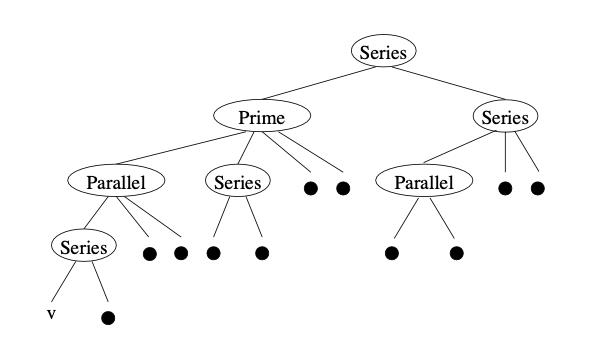
\includegraphics[width=0.80\textwidth]{images/graphs/modular-decomposition-tree}
    \caption{A modular decomposition tree}
    \label{fig:example-modular-decomposition-tree}
\end{figure}

\begin{algorithm}[H]
    \caption{Ehrenfeucht et al. \cite{SAMD}\cite{PTDMD}} % Reference citation in the caption
    \KwIn{An arbitrary vertex $v$ of $G = (V, E)$, $T = \text{spine}(G, v)$ and $\{T_X = MD(G[X]) \mid X \in \mathcal{M}(G,v)\}$}
    \KwOut{The modular decomposition tree $MD(G)$}
    \SetKwBlock{Begin}{begin}{end}
    \Begin{
        \ForEach{leaf $X$ of $T$}{
            Let $T_X = MD(G[X])$ and $p(X)$ be $X$'s father in $T$\; \\
            Replace $X$ by $T_X$ in $T$\;
            \If{the root $r(T_X)$ and $p(X)$ are both parallel or series}{
                Remove $r(T_X)$ and connect the children of $r(T_X)$ to $p(X)$\;
            }
        }
    }\label{alg:algorithm-Ehrenfeucht-et-al}
\end{algorithm}


\section{Example of application}\label{sec:example-of-application}

Consider a simple graph $G$ with vertices $V = \{1, 2, 3, 4, 5\}$ and edges $E = \{\{1, 2\}, \{1, 3\}, \{2, 3\}, \{4, 5\}\}$.
The modular decomposition using Ehrenfeucht's algorithm can be illustrated as follows:

\begin{enumerate}
    \item \textbf{Choose Pivot Vertex}:
            \begin{itemize}
                \item Select vertex $1$ as the pivot.
            \end{itemize}
    \item \textbf{Partition the Graph}:
            \begin{itemize}
                \item Partition $\{2, 3, 4, 5\}$ based on their adjacency to $1$:
                        \begin{itemize}
                            \item $2$ and $3$ are adjacent to $1$.
                            \item $4$ and $5$ are not adjacent to $1$.
                        \end{itemize}
                \item Resulting modules: $\{2, 3\}$ and $\{4, 5\}$.
            \end{itemize}
    \item \textbf{Recursive Decomposition}:
            \begin{itemize}
                \item Apply the algorithm to the subgraphs induced by $\{2, 3\}$ and $\{4, 5\}$:
                        \begin{itemize}
                            \item Subgraph $\{2, 3\}$ is already fully connected (a prime module).
                            \item Subgraph $\{4, 5\}$ is also fully connected (a prime module).
                        \end{itemize}
            \end{itemize}
    \item \textbf{Construct Modular Decomposition Tree}:
            \begin{itemize}
                \item Combine the results to form the modular decomposition tree: ('COMPLETE', [('COMPLETE', [1, ('COMPLETE', [2, 3])]), ('COMPLETE', [4, 5])])
            \end{itemize}
\end{enumerate}


\section{Advantages of Ehrenfeucht's Algorithm}\label{sec:advantages-of-ehrenfeucht's-algorithm}

\begin{itemize}
    \item \textbf{Efficiency:} The algorithm operates in $O(n + m\log{n})$ time, making it feasible for large graphs.
    \item \textbf{Simplicity:} The divide-and-conquer approach simplifies the process of identifying modules and constructing the decomposition tree.
    \item \textbf{Practicality:} The algorithm is applicable to both undirected graphs and 2-structures.
\end{itemize}


\hspace{4cm}

The next chapter will discuss an implementation of the algorithm in Python made by another Sorbonne University student and its performance compared with another implementation made in SageMath.
